\documentclass[a4paper]{article}
\usepackage[utf8]{inputenc}
\usepackage[T1]{fontenc}
\usepackage[finnish]{babel}
\usepackage{geometry}
\usepackage{graphicx}
\usepackage{url}


\begin{document}

\section*{Tietokantasovellus, harjoitustyö}
\section{Johdanto}

Harjoitustyön aiheena drinkkiarkisto. Tarkoituksena on luoda drinkkireseptien hakulomake, jota käytetään www-sivulla. Lomakkeeseen kirjaudutaan sisään, ja sillä eri reseptejä voi hakea ja listata. Listauksessa reseptejä voi laittaa järjestykseen monella eri tapaa, esimerkiksi ne voi järjestää jonkin tietyn reseptin ainesosan mukaan. Resepteihin voidaan viitata monilla eri hakusanoilla, ja yhdellä hakusanalla voi saada useamman tuloksen. 

Lomakkeella on ylläpitäjä tai ylläpitäjiä sekä tavallisia käyttäjiä. Tavallinen käyttäjä voi ehdottaa reseptin lisäystä tietokantaan. Ylläpitäjä voi hyväksyä ehdotuksen, ja lisätä reseptin joko tiedostosta tai lomakkeella. Ylläpitäjä voi myös antaa ylläpito-oikeudet tavalliselle käyttäjälle. 

Tietokantana on PostgreSQL. Harjoitustyö toteutetaan laitoksen user--palvelimella PHP-kielellä. 

%Johdantoon kirjoitetaan lyhyt, ytimekäs kuvaus siitä, mikä on työn aihe, mitä työllä kuuluisi pystyä tekemään ja mitä tekniikoita siinä käytetään.
%
%Järjestelmän tarkoitus
%Tiivis kuvaus siitä mistä on kyse.
%Millaisen toiminnan tukemiseen järjestelmä on tarkoitettu.
%Mitkä ovat järjestelmän tavoitteet.
%Nämä tiedot saa yleensä tehtäväkuvauksesta, kirjoita kuitenkin omin sanoin.

%Toteutus-/toimintaympäristö
%Missä ympäristössä työ toteutetaan (yleensä laitoksen users-palvelimella Tomcat- tai Apache-palvelimen alla)
%Täytyykö web-sovelluksen alustajärjestelmän tukea jotain tiettyä ohjelmointikieltä. (esim. Java, Ruby, PHP..?)
%Jos edellytetään jotain sovelluskehystä tulisi sekin mainita.
%Täytyykö käyttäjän selaimen tukea jotain tiettyä ohjelmointikieltä (esim. javascript?).
%Edellyttääkö ohjelmisto jonkun tietyn tietokannan käyttöä vai voiko sitä vaihtaa helposti. Useimmat työt toimivat vain yhdellä kannalla.
\section{Käyttäjistä}

\subsection{Käyttötapauskaavio}
\begin{figure}[h]
	\centering
	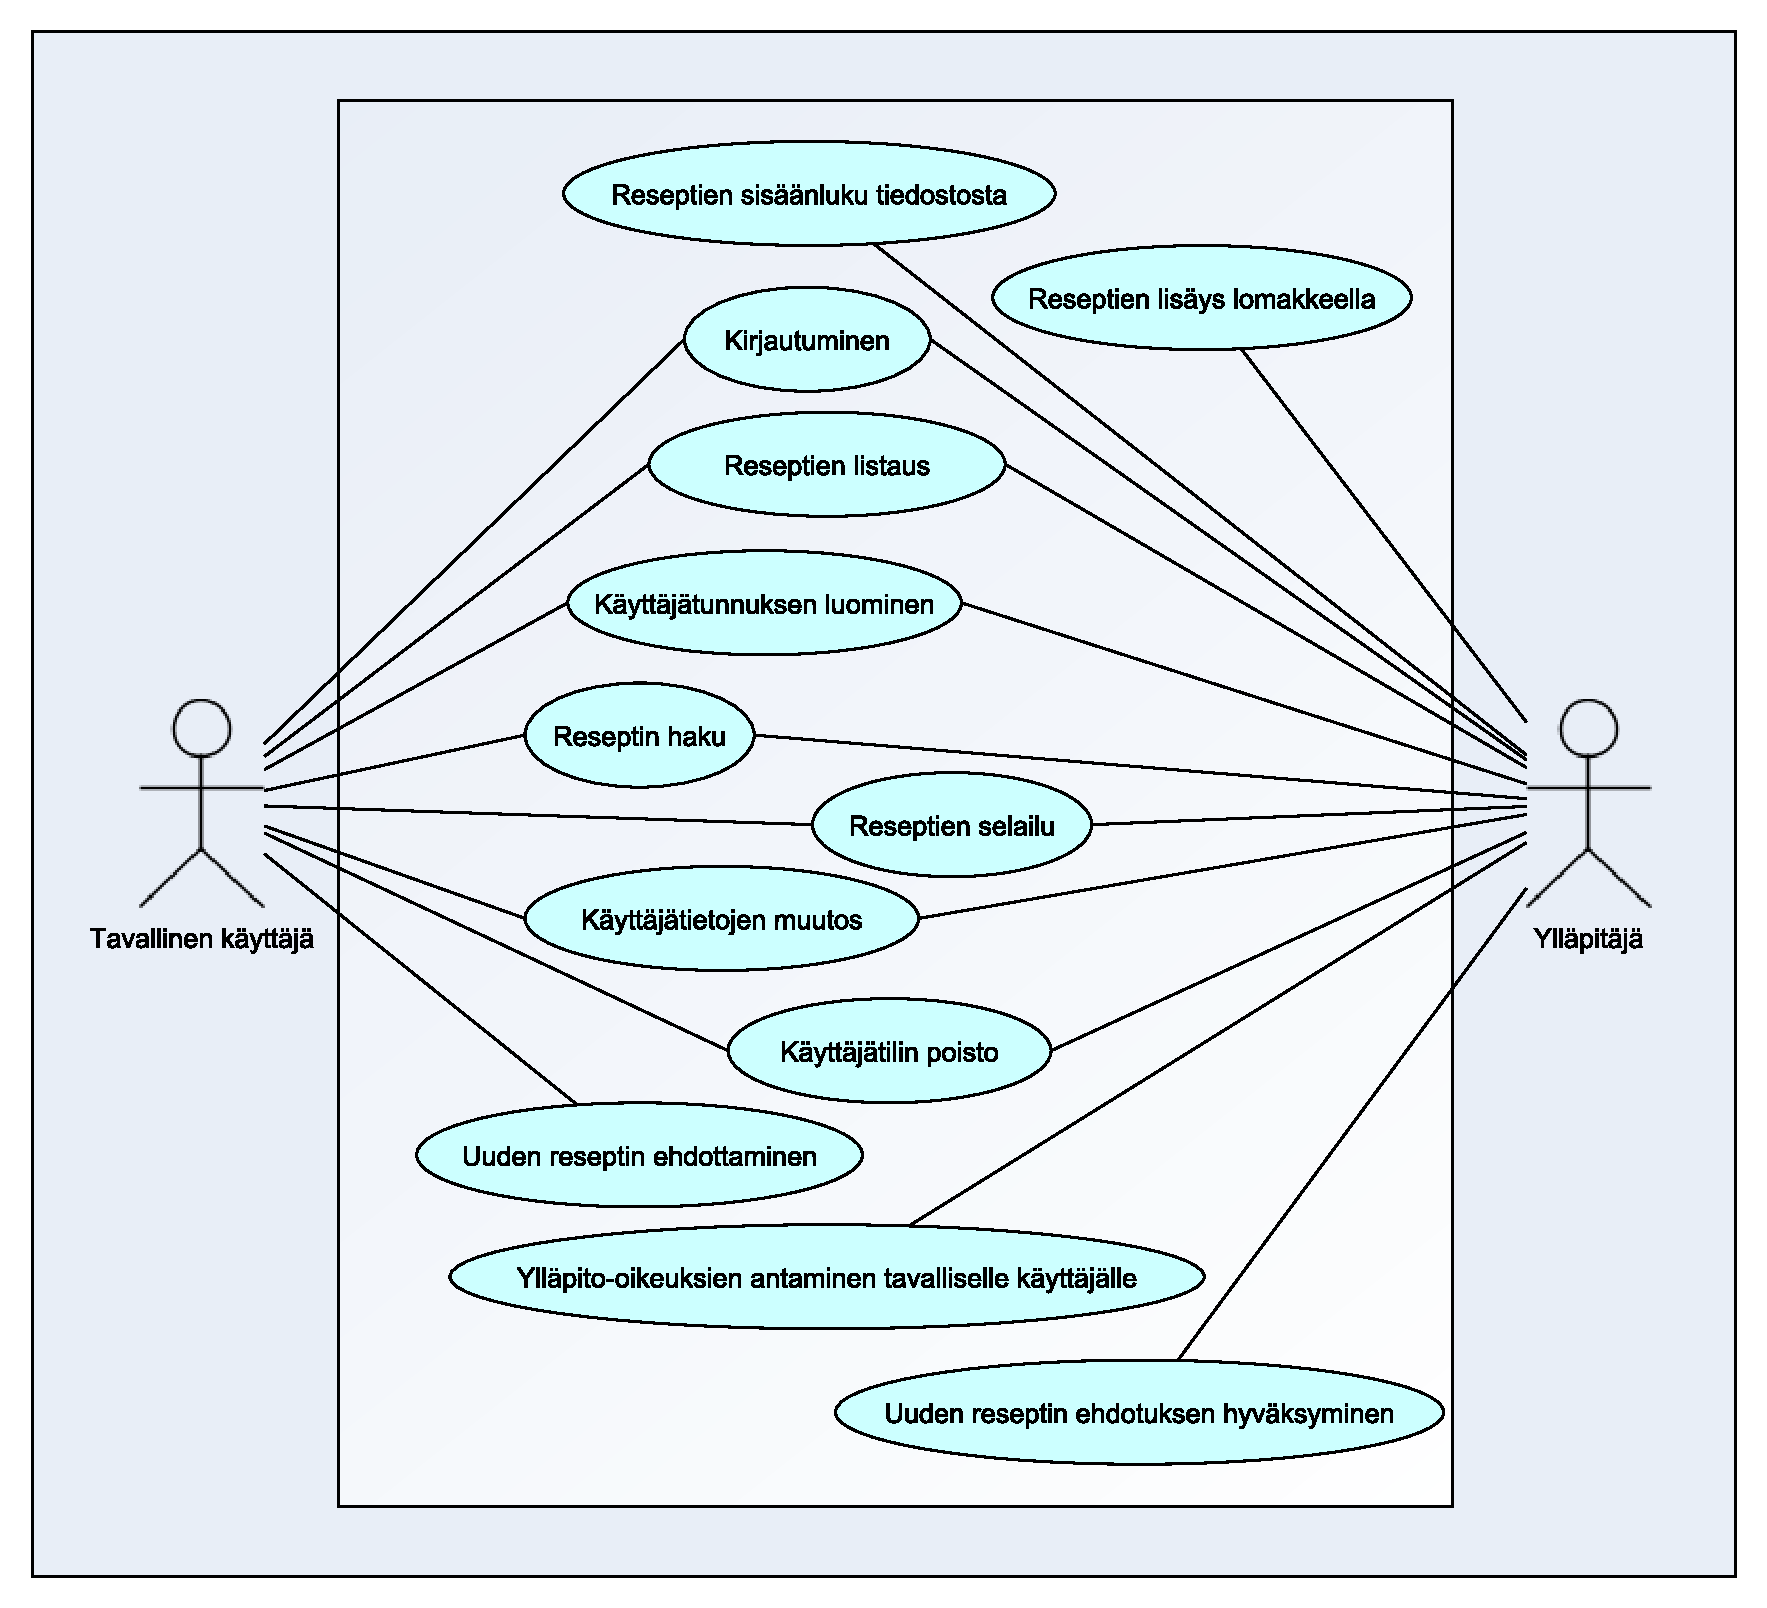
\includegraphics[scale=0.4]{kayttotapaukset.pdf}
	\caption{Käyttötapauskaavio}
\end{figure}
	
\subsection{Käyttäjäryhmät}

\begin{flushleft}Ylläpitäjä\end{flushleft}

Ylläpitäjän pitää olla rekisteröitynyt lomakkeen käyttäjä, jolle on annettu ylläpito-oikeudet. Lomake vaatii sisäänkirjautumisen.

\begin{flushleft}Tavallinen käyttäjä\end{flushleft}

Tavallinen käyttäjä voi olla kuka tahansa sivulle kirjautunut henkilö. 

\subsection{Käyttötapaukset}

\begin{flushleft}\textbf{Ylläpitäjä\(\colon\)} \end{flushleft}
\begin{itemize}
	\item Reseptien haku\(\colon\) käyttäjä voi hakea tietokannasta reseptejä hakusanalla. Yksi hakusana voi tuottaa monta tulosta.
	\item Reseptien listaus\(\colon\) käyttäjä voi listata reseptit ainesosan mukaan tai aakkos-- tai juomalajijärjestykseen.
	\item Ylläpito-oikeuden antaminen tavalliselle käyttäjälle\(\colon\) käyttäjä voi tehdä tavallisesta käyttäjästä ylläpitäjän. 
	\item Uuden reseptin ehdotuksen hyväksyminen\(\colon\) käyttäjä voi hyväksyä tavallisen käyttäjän reseptiehdotuksen, ja lisätä reseptin tietokantaan.
	\item Reseptin lisäys lomakkeella\(\colon\) käyttäjä voi lisätä reseptin käyttäen siihen tarkoitettua lomaketta.
	\item Reseptin lisäys tiedostosta\(\colon\) käyttäjä voi lisätä uuden reseptin lukemalla sen suoraan tiedostosta. 
	\item Muut käyttötapaukset\(\colon\) Käyttäjätietojen muutos, käyttäjätilin poisto, käyttäjätunnuksen luominen, reseptien selaaminen, kirjautuminen
\end{itemize}

\begin{flushleft}\textbf{Tavallinen käyttäjä\(\colon\)} \end{flushleft}

\begin{itemize}
	\item Reseptien haku \(\colon\) käyttäjä voi hakea tietokannasta reseptejä hakusanalla. Yksi hakusana voi tuottaa monta tulosta.
	\item Reseptien listaus\(\colon\) käyttäjä voi listata reseptit ainesosan mukaan tai aakkos-- tai juomalajijärjestykseen.
	\item Uuden reseptin ehdottaminen\(\colon\) käyttäjä voi ehdottaa uutta reseptiä ylläpitäjälle lisättäväksi tietokantaan.
	\item Muut käyttötapaukset\(\colon\) Käyttäjätietojen muutos, käyttäjätilin poisto, käyttäjätunnuksen luominen, reseptien selaaminen, kirjautuminen
\end{itemize}

\section{Järjestelmän tietosisältö}
\begin{flushleft}\textbf{Käsitekaavio} \end{flushleft}

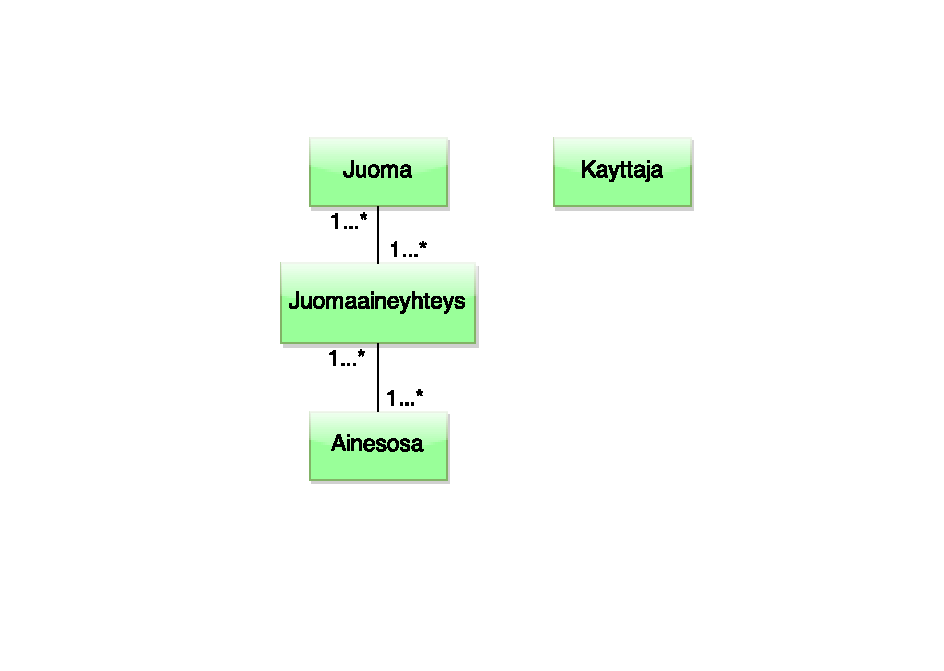
\includegraphics[scale=0.8]{kasitekaavio.pdf}

\begin{flushleft}\textbf{Juoma} \end{flushleft}
\begin{flushleft}
	\begin{tabular}{|l|l|l|}\hline
			Attribuutti      & Arvojoukko        & Kuvailu\\
			\hline
			nimi & merkkijono, maksimissaan 50 merkkiä & Juoman nimi.\\ 
			\hline
			lisääjä & merkkijono, maksimissaan 50 merkkiä & Lisääjän nimimerkki.\\ 
			\hline
			lisäyspäivämäärä & päivämäärä (date) & Päivämäärä, jolloin drinkkiohje on lisätty.\\ 
			\hline
			ainesosat  & merkkijono,maksimissaan 50 merkkiä & Ainekset, joista drinkki tehdään. \\
			\hline
			juomalaji    & merkkijono,maksimissaan 50 merkkiä  & Juoman käyttötarkoitus. \\ 
			\hline
			kuvaus    & merkkijono, maksimissaan 400 merkkiä & Juoman kuvaus. \\ 
				\hline
	\end{tabular}
\end{flushleft}

\begin{flushleft}\textbf{Ainesosat} \end{flushleft}
\begin{flushleft}
	\begin{tabular}{|l|l|l|}
			\hline
			Attribuutti & Arvojoukko & Kuvailu \\ 
			\hline
			ainesosa & merkkijono, maksimissaan 50 merkkiä & Ainesosan nimi. \\ 
			\hline
	\end{tabular}
\end{flushleft}

\begin{flushleft}\textbf{Käyttäjä} \end{flushleft}
\begin{flushleft}
	\begin{tabular}{|l|l|l|}
			\hline
			Attribuutti & Arvojoukko & Kuvailu   \\ 
			\hline
			nimimerkki  & merkkijono, maksimissaan 50 merkkiä & Käyttäjän nimimerkki. \\ 
			\hline
			salasana    & merkkijono, maksimissaan 50 merkkiä & Käyttäjän salasana.   \\ 
			\hline
	\end{tabular}
\end{flushleft}

\begin{flushleft}\textbf{Ainesosayhteys} \end{flushleft}
\begin{flushleft}
	\begin{tabular}{|l|l|l|}
			\hline
			Attribuutti & Arvojoukko & Kuvailu   \\ 
			\hline
			juoma id  & lukujono & Yhteys Juoma-tauluun. \\ 
			\hline
			ainesosa id    & lukujono & Yhteys Ainesosa-tauluun.  \\ 
			\hline
	\end{tabular}
\end{flushleft}

\section{Relaatiokaavio}
\begin{flushleft}\textbf{Relaatiokaavio} \end{flushleft}

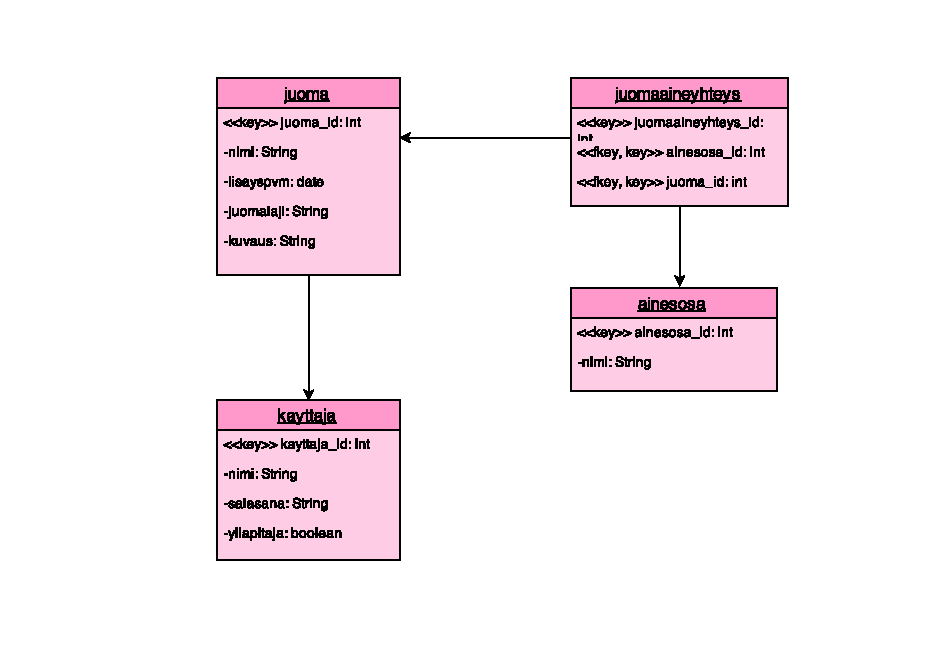
\includegraphics[scale=0.8]{relaatiokaavio.pdf}


\section{Järjestelmän yleisrakenne}
\section{Käyttöliittymä ja järjestelmän komponentit}
\section{Asennustiedot}
\section{Käynnistys- /käyttöohje}
Harjoitustyö löytyy osoitteesta \url{http://kaem.users.cs.helsinki.fi/Drinkkiarkisto/}


Kirjautumiseen tarvittava käyttäjätunnus on xxxx ja salasana xxxx.
\section{Testaus, tunnetut bugit ja puutteet ja jatkokehitysideat}
\section{Omat kokemukset}
\section{Muu dokumentaatio}

\end{document}
